% !TeX program = lualatex
% ================================================================
% Polish Tier 3 Vocabulary Version of RatioAndProportionBooklet
%
% Generated by the server using the following settings:
%
%   language            Polish (pol)
%   text direction      left to right
%   font                Noto Serif
%   fallback font       Noto Serif
%   built from          latex/worksheets/ratioAndProportion/ratioAndProportionBooklet.tex
%   vocabulary key      latex/worksheets/ratioAndProportion/ratioAndProportionBooklet/L2/pol/ratioAndProportionBooklet_polishKey.tex
%   tier 3 vocabulary   green   RGB 0 128 0
%   English text        black   RGB 0 0 0
%   Polish text         purple  RGB 112 48 160
%   layout macros       version 3
%
% Please don't edit any information in this comment block - the server
% compares it against the current settings and rebuilds this file when
% they differ, so changes here would be overwritten. However, feel free
% to make updates to the LaTeX below if you want to edit it.
% ================================================================

\documentclass[12pt,a4paper]{article}
% ================================================================
% Copied from the English sheet this was translated from, so that
% anything it sets up for itself still works here
% ================================================================
\usepackage{amsmath} % For advanced math formatting
\usepackage{tikz} % For drawing diagrams
\usepackage{geometry} % For adjusting page margins
\geometry{margin=1in}
\usetikzlibrary{shapes.geometric, arrows.meta, positioning}
\usepackage{enumitem} % For customising lists
\usepackage{siunitx} % For units

\pagenumbering{gobble} 

\title{ImprovementActivitySheetsCore}
\author{matthew.holmes111 }
\date{November 2025}

% Characters this language's font has not got are borrowed from another,
% rather than being silently dropped - see docs/translated-sheet-latex.md
\directlua{%
  if luaotfload and luaotfload.add_fallback then
    luaotfload.add_fallback("eallatinfallback",
      { "Noto Serif:mode=harf;" })
  else
    tex.error("this luaotfload is too old to register a fallback font")
  end
}
\usepackage[english]{babel}
\babelprovide[import]{polish}
\babelfont[polish]{rm}[Renderer=Harfbuzz, BoldFont={Noto Serif}, ItalicFont={Noto Serif}, BoldItalicFont={Noto Serif}, RawFeature={fallback=eallatinfallback}]{Noto Serif}
\babelfont[polish]{sf}[Renderer=Harfbuzz, BoldFont={Noto Serif}, ItalicFont={Noto Serif}, BoldItalicFont={Noto Serif}, RawFeature={fallback=eallatinfallback}]{Noto Serif}
\newcommand{\ealtext}[1]{\foreignlanguage{polish}{#1}}
\newcommand{\ealtextblock}[1]{{\raggedright\foreignlanguage{polish}{#1}\par}}
% ================================================================
% EAL layout helpers
% ================================================================
\usepackage{xcolor}

\definecolor{ealkeycolour}{RGB}{0,128,0}
\definecolor{ealenglish}{RGB}{0,0,0}
\definecolor{ealtwocolour}{RGB}{112,48,160}

\newsavebox{\ealboxen}
\newsavebox{\ealboxtr}
\newlength{\ealglosswd}
\newlength{\ealglossraise}
\setlength{\ealglossraise}{1.15em}

% a tier 3 word, in English and in translation alike
\newcommand{\ealkey}[1]{\textcolor{ealkeycolour}{#1}}
\newcommand{\ealkeytr}[1]{\textcolor{ealkeycolour}{\ealtext{#1}}}

% One translated word above one English word. Built from kernel
% primitives, never a tabular, which would break wherever the sheet
% loads array, booktabs or tabularx. The box is as wide as the wider of
% the two, so a long translation pushes its neighbours aside instead of
% overlapping them, and it claims its full height so a table row or a
% TikZ node makes room for it.
\newcommand{\ealgloss}[2]{%
  \sbox{\ealboxen}{\ealkey{#1}}%
  \sbox{\ealboxtr}{\small\textcolor{ealtwocolour}{\ealtext{#2}}}%
  \setlength{\ealglosswd}{\wd\ealboxen}%
  \ifdim\wd\ealboxtr>\ealglosswd\setlength{\ealglosswd}{\wd\ealboxtr}\fi
  \leavevmode
  \makebox[\ealglosswd][c]{%
    \makebox[0pt][c]{\usebox{\ealboxen}}%
    \makebox[0pt][c]{\raisebox{\ealglossraise}{\usebox{\ealboxtr}}}%
  }%
}

% opens up line spacing around a block of glosses, so the raised
% translations sit clear of the line above
\newenvironment{ealglossed}{\par\linespread{2.1}\selectfont\ignorespaces}{\par}

% a whole translated sentence above its English counterpart. block level,
% so it does not belong inside a tabular cell
\newcommand{\ealpara}[2]{%
  \par\addvspace{0.5\baselineskip}%
  {\color{ealtwocolour}\ealtextblock{#1}}%
  \penalty200
  {\color{ealenglish}#2\par}%
  \addvspace{0.5\baselineskip}%
}

\begin{document}

\begin{ealglossed}
\section*{Simplifying \ealgloss{Ratios}{stosunki}}
\end{ealglossed}

\begin{ealglossed}
\emph{Simplify these \ealgloss{ratios}{stosunki} to their \ealgloss{simplest form}{najprostsza postać}.}
\end{ealglossed}

\begin{enumerate}
\item \( 14 : 21 \)

\vspace{0.8cm}

\item \( 24 : 18 : 42 \)

\vspace{0.8cm}

\item \( 1.5 : 4.5 \)

\vspace{0.8cm}

\item \( \frac{2}{3} : \frac{4}{5} \)

\vspace{0.8cm}

\item \begin{ealglossed} A recipe for paint mix requires 600 ml of white paint, 250 ml of blue paint, and 150 ml of yellow paint. What is the \ealgloss{ratio}{stosunek} of white : blue : yellow paint in its \ealgloss{simplest form}{najprostsza postać}? \end{ealglossed}

\vspace{1.2cm}
\end{enumerate}

\vspace{3cm}

\begin{ealglossed}
\section*{Sharing into \ealgloss{Ratios}{stosunki}}
\end{ealglossed}

Divide the quantities as described.

\begin{enumerate}
    \item \begin{ealglossed} Share 24 sweets between two children in the \ealgloss{ratio}{stosunek} 3:1. \end{ealglossed}

    \item \begin{ealglossed} An amount of £80 is divided between two people in the \ealgloss{ratio}{stosunek} 3:2. How much does each person receive? \end{ealglossed}

    \item \begin{ealglossed} 180 students are divided into three groups in the \ealgloss{ratio}{stosunek} 2:3:4. How many students are in each group? \end{ealglossed}

    \item \begin{ealglossed} A piece of wood 2.4 meters long is cut into three pieces in the \ealgloss{ratio}{stosunek} 1:2:5. Find the length of each piece. \end{ealglossed}

    \item \begin{ealglossed} A bag contains red, blue, and green marbles in the \ealgloss{ratio}{stosunek} 2:5:3. If there are 150 marbles in total, how many of each color are there? \end{ealglossed}
\end{enumerate}

\newpage{}

\section*{Recipe Questions}

\begin{enumerate}
\item A recipe for 4 servings requires:
    \begin{itemize}
    \item 400g minced beef
    \item 2 onions (300g)
    \item 400g chopped tomatoes
    \item 150ml stock
    \end{itemize}
    How much of each ingredient is needed to make 10 servings?

\item A cookie recipe makes 15 cookies:
    \begin{itemize}
    \item 225g flour
    \item 150g butter
    \item 100g sugar
    \item 1 egg (50g)
    \end{itemize}
    How much of each ingredient is needed to make 35 cookies?

\item A salad dressing recipe for 2 portions:
    \begin{itemize}
    \item 60ml olive oil
    \item 30ml vinegar
    \item 10g mustard
    \item 5g honey
    \end{itemize}
    You need to make dressing for 7 portions. Calculate the new quantities.

\item \begin{ealglossed} The ingredients for a lemonade are in the \ealgloss{ratio}{stosunek} of \newline lemon juice : sugar : water = 2 : 1 : 8. To make 3.3 litres of lemonade, what volume of each ingredient is needed? \end{ealglossed}

\item A curry recipe for 4 people calls for:
    \begin{itemize}
    \item 400g chicken
    \item 200g rice
    \item 300ml coconut milk
    \item 6 spices (individual items)
    \end{itemize}
    \begin{enumerate}
    \item Calculate the ingredient quantities needed to serve 11 people.
    \item You discover you only have 600g of chicken. What is the maximum number of people you can fully serve?
    \item Using the chicken from part (b), calculate the quantities for all other ingredients.
    \end{enumerate}
\end{enumerate}

\newpage{}

\begin{ealglossed}
\section*{Direct \ealgloss{Proportion}{proporcjonalność}}
\end{ealglossed}

\begin{enumerate}
    \item If 4 pencils cost 96p, find the cost of 7 pencils.

    \item \begin{ealglossed} A car travels 180 km in 3 hours. Assuming a \ealgloss{constant}{stała} \ealgloss{speed}{prędkość}, how far will it travel in 7 hours? \end{ealglossed}

    \item The amount of paint needed is directly proportional to the area painted. If 2 litres of paint can cover 15 m$^2$, how many litres are needed to cover 90 m$^2$?

    \item The cost of a piece of rope is directly proportional to its length. A 2.5 metre piece of rope costs £1.35. Bob buys a piece of this rope and the cost is £3.24. What is the length of the rope he bought?

    \item The mass of a uniform metal bar is directly proportional to its length. A 1.2 m long bar has a mass of 4.5 kg. What is the mass of a similar bar that is 80 cm long?
\end{enumerate}

\vspace{6cm}


\section*{Best Buys}

\begin{enumerate}
\item Which is cheaper per gram: 200g of coffee for £5.40 or 350g for £8.75?

\item Pencils cost £4.80 for a pack of 12 or £11.00 for a pack of 30. Which pack offers better value per pencil?

\item Milk costs £2.85 for 2 liters or £6.50 for 5 liters. Which is the better buy?

\item A restaurant needs to buy rice. Option A: 8kg for £24.80. Option B: 15kg for £44.25. Option C: 25kg for £72.50. Which offers the best value per kilogram?

\item A car rental company charges: \\
Company X: £45 per day with unlimited mileage \\
Company Y: £35 per day plus £0.15 per mile \\
If you plan to drive 250 miles over 3 days, which company offers the better deal?
\end{enumerate}

\newpage{}

\begin{ealglossed}
\section*{\ealgloss{Scaling}{skalowanie}}
\end{ealglossed}

\begin{enumerate}

\item \begin{ealglossed} A \ealgloss{scale}{skalować} drawing uses a \ealgloss{ratio}{stosunek} of 1:100. If a wall is drawn as 3.5 cm long, how long is the actual wall? \end{ealglossed}

\item \begin{ealglossed} On a map with \ealgloss{scale}{skalować} 1:50,000, two towns are 8.4 cm apart. What is the actual distance between them in kilometres? \end{ealglossed}

\item 
\begin{ealglossed}
If the rectangle below represents a garden drawn to \ealgloss{scale}{skalować} 1:20, and it measures 4 cm by 3 cm in the drawing, what are the actual dimensions of the garden?
\end{ealglossed}
\begin{ealglossed}
\begin{center}
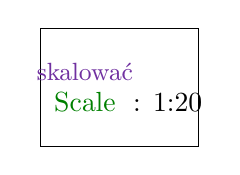
\begin{tikzpicture}[scale=0.5]
\draw (0,0) rectangle (4,3);
\node at (2,1.5) {\ealgloss{Scale}{skalować}: 1:20};
\end{tikzpicture}
\end{center}
\end{ealglossed}

\item \begin{ealglossed} James is making a \ealgloss{scale}{skalować} model of a car. The actual car is 4.2 meters long, and his model is 28 cm long. What \ealgloss{scale}{skalować} is he using? Express your answer as a \ealgloss{ratio}{stosunek} in \ealgloss{simplest form}{najprostsza postać}. \end{ealglossed}

\item \begin{ealglossed} A map has a \ealgloss{scale}{skalować} where 4 cm represents 5 km. Two cities appear 15.2 cm apart on the map. \end{ealglossed}
\begin{enumerate}
    \item What is the actual distance between the cities?
    \item \begin{ealglossed} What is the map \ealgloss{scale}{skalować} expressed as a \ealgloss{ratio}{stosunek}? \end{ealglossed}
    \item \begin{ealglossed} If another map uses \ealgloss{scale}{skalować} 1:125,000, which map shows more detail (larger \ealgloss{scale}{skalować})? \end{ealglossed}
\end{enumerate}

\item \begin{ealglossed} The floor plan of a small room is 6 meters long and 4.5 meters wide. Using the squared background below, create a \ealgloss{scale}{skalować} drawing of this room. Use a \ealgloss{scale}{skalować} of \newline 1 cm : 1 m. Clearly label the dimensions on your drawing. \end{ealglossed}
\begin{center}

\begin{tikzpicture}
\draw[step=1cm, gray, very thin] (0,0) grid (10,7);
\end{tikzpicture}
\end{center}

\end{enumerate}

\newpage{}

\begin{ealglossed}
\section*{\ealgloss{Rates}{wielkości ilorazowe} of Change}
\end{ealglossed}

\begin{enumerate}
    \item \begin{ealglossed} A cyclist travels \SI{45}{\kilo\metre} in 1 hour and 30 minutes. Calculate her \ealgloss{average}{średnia} \ealgloss{speed}{prędkość} in \si{\kilo\metre\per\hour}. \end{ealglossed}

    \item \begin{ealglossed} Water flows from a tap at a \ealgloss{constant}{stała} \ealgloss{rate}{wielkość ilorazowa}. It takes 3 minutes to fill a \SI{12}{\litre} watering can. At this \ealgloss{rate}{wielkość ilorazowa}, how long would it take to fill a \SI{90}{\litre} water butt? \end{ealglossed}

    \item \begin{ealglossed} A train leaves London at 10:15 and arrives in York, \SI{320}{\kilo\metre} away, at 14:45. It stops for 10 minutes at a station halfway through the journey. Calculate the train's \ealgloss{average}{średnia} \ealgloss{speed}{prędkość} for the whole journey, \textbf{including} the stop. What about the \ealgloss{average}{średnia} \ealgloss{speed}{prędkość} when the train was in motion? \end{ealglossed}

    \item \begin{ealglossed} A chemical reaction happens in a beaker. At the start, the beaker contains \SI{400}{\gram} of chemical A. The reaction uses up A at a \ealgloss{rate}{wielkość ilorazowa} of 4 grams per minute, how much chemical A is left in the beaker after 4 minutes? \end{ealglossed}

    \item \begin{ealglossed} Sarah is driving on a motorway. She drives for \SI{30}{\minute} at an \ealgloss{average}{średnia} \ealgloss{speed}{prędkość} of \SI{60}{\text{miles}\per\hour}. She then stops at a service station for 15 minutes. She completes her journey by driving for another \SI{45}{\minute} at an \ealgloss{average}{średnia} \ealgloss{speed}{prędkość} of \SI{50}{\text{miles}\per\hour}. \end{ealglossed}
    \begin{enumerate}
        \item Calculate the total distance of her journey.
        \item \begin{ealglossed} Calculate her \ealgloss{average}{średnia} \ealgloss{speed}{prędkość} for the \textbf{whole journey}, including the stop. \end{ealglossed}
    \end{enumerate}

\end{enumerate}

\vspace{3cm}

\begin{ealglossed}
\section*{Problem Solving With \ealgloss{Ratios}{stosunki}}
\end{ealglossed}
\begin{enumerate}

    \item \begin{ealglossed} The \ealgloss{ratio}{stosunek} of red to blue marbles in a bag is $3:5$. If 8 red marbles are added, the \ealgloss{ratio}{stosunek} becomes $5:7$. How many blue marbles are there? \end{ealglossed}

    \item \begin{ealglossed} The \ealgloss{ratio}{stosunek} of apples, bananas, and oranges in a fruit basket is $2:5:3$. After 4 apples and 2 bananas are added, the new \ealgloss{ratio}{stosunek} of apples to bananas to oranges is $4:6:3$ How many oranges are in the basket? \end{ealglossed}

    \item \begin{ealglossed} The \ealgloss{ratio}{stosunek} of sugar to flour in a recipe is $2:9$. The \ealgloss{ratio}{stosunek} of flour to butter is $3:1$. Find the \ealgloss{ratio}{stosunek} of sugar to flour to butter. \end{ealglossed}

    \item \begin{ealglossed} A sum of money is divided between Alex, Ben, and Chloe in the \ealgloss{ratio}{stosunek} $3:4:5$. If Ben receives £40 more than Alex, find the total sum of money. \end{ealglossed}

    \item \begin{ealglossed} The points $A$, $B$, and $C$ lie on a straight line. The \ealgloss{ratio}{stosunek} of $AB$ to $BC$ is $3:2$. If $AB = 12$ cm, find the length of $AC$. \end{ealglossed}

    \item \begin{ealglossed} A bag contains counters in three colours: red, yellow, and blue. The \ealgloss{ratio}{stosunek} of red to yellow is $3:4$. The \ealgloss{ratio}{stosunek} of yellow to blue is $5:6$. What \ealgloss{fraction}{ułamek} of the counters are blue? \end{ealglossed}

    \item \begin{ealglossed} The \ealgloss{ratio}{stosunek} of red to blue marbles in a bag is $2:3$. After $36$ red marbles, and $29$ blue marbles are added the \ealgloss{ratio}{stosunek} becomes $4:5$. How many blue marbles were in the bag initially? \end{ealglossed}

\end{enumerate}

\end{document}